\documentclass[12pt]{article}

\usepackage[margin=1.4in]{geometry}
\usepackage{amsmath}
\usepackage{graphicx}
\graphicspath{{./figures/}}

\begin{document}
\begin{titlepage}

\begin{center}
\begin{huge}
Audio Compression\\
\end{huge}
14-bit to 8-bit\\
\vspace{1.5cm}
\textbf{Duncan MacDonald}\\
duncmac.16@gmail.com\\
V00842740\\
\vfill
SENG 440 - Embedded Systems\\
University Of Victoria\\
Department of Engineering\\
\vspace{1.5cm}
\today
\end{center}
\end{titlepage}
\newpage
\tableofcontents
\newpage
\section{Introduction}
\indent 
Recording audio and storing it digitally, in its fullest form is a very costly process; the same goes for transmitting it. For that reason, audio compression came to be. There are two type of audio compression methods, lossless and lossy, this report will be going over the latter, specifically $\mu$-law and $A$-law. Even though $\mu$-law does loss some data in compression, it's usage is still justified in telecommunication as it makes data transfer a lot faster with little noticeable to the human ear[1].\\

$\mu$-law takes in a 14-bit sample (14 of which are used) of the recorded signal and creates a logarithmic approximation of the signal recording the position of the most significant bits and the step of the preceding bits. This project in particular is an implementation of $\mu$-law used on to compress a audio file and uses the inverse to expand it back to a usable file. After the initial implementation was create, multiple different optimization techniques were preformed to the algorithm to take the highest traffic parts and reduce the instructions needed to complete them. After the software optimizations were completed, hypothetical hardware assisted were added to the algorithm to increase the speed of the algorithm even further.\\

The resulting algorithm would be the base to a highly optimized embedded system could be further implemented with hardware to be used in a production setting. The following report highlights the background knowledge the algorithm is based on, the optimization techniques used in the software and performance analysis on all stages of the design.\\
 
\section{Background}

The basis of why the data lost in compression is justifiable is the characteristics of human speech[1]. Most of the things people say vocally are of a much higher amplitude than things such as background noise or sounds of friction of things around the recording device[1]. This is why compressing large signals of vocal sounds is affordable, since the lower amplitude signals of non-vocal sounds aren't really relevant to the transfer of human voice. \\

The way that wave files are recorded is in uniformly spaced quantized values of a signal, with lower levels of noise recorded with fewer bits and larger levels of noise recorded with more bits. This is referred to as uniform pulse code modulation[1]. The idea behind such codec as $\mu$-law and $A$-law is to take a logarithmic representation of the uniformly spaced signals so that an 8-bit code can represent the potentially larger signal. \\

\begin{align}
y = sgn(x)\frac{ln(1+\mu|x|)}{ln(1+ \mu)}\\
y = \begin{cases}
sgn(x)\frac{A|x|}{1+ln A} \\
sgn(x)\frac{1+ln(A|x|)}{1 + ln A}\\
\end{cases}
\end{align}

$\mu$-law, represented by equation 1 is the function that is to implemented in software, where $\mu$ is a parameter that can range from 0 (no compression) to 255 (maximum compression)[1]. To implement this in software, I am going to use a piecewise logarithmic approximation of this equation to compress a signal. Inversely, I am going to use exponentials to expand the compressed codec into something useful again. \\
\section{Design}

For a design methodology, I used a low cost version of test driven development. To produce some samples I made a 16-bit integer as a pseudo-sample and compressed it into a code word and expanded it again. In the end of the first iteration, some of the samples produced by the testing did not expand back in the same format, but it was expected since the samples produced were not in the format of a 14-bit quantized value. The rest of the values expanded in a similar fashion, only keeping the five or six most significant figures and dropping the rest. The samples produced were dispersed throughout a range of different chords and steps so that all aspects were tested. I used a for loop as seen in figure 1 that takes the initial sample and shifts it over one space, clearing the most significant bit and compresses and decompresses sample and displays the results. This was then repeat with a different step to ensure that the steps were correctly being compressed. As I mentions before this was a low cost testing method, so no actual testing software was used. Using a form of test driven development was very helpful though, as bugs that occurred were quickly seen and corrected.\\

\begin{figure}[!h]
        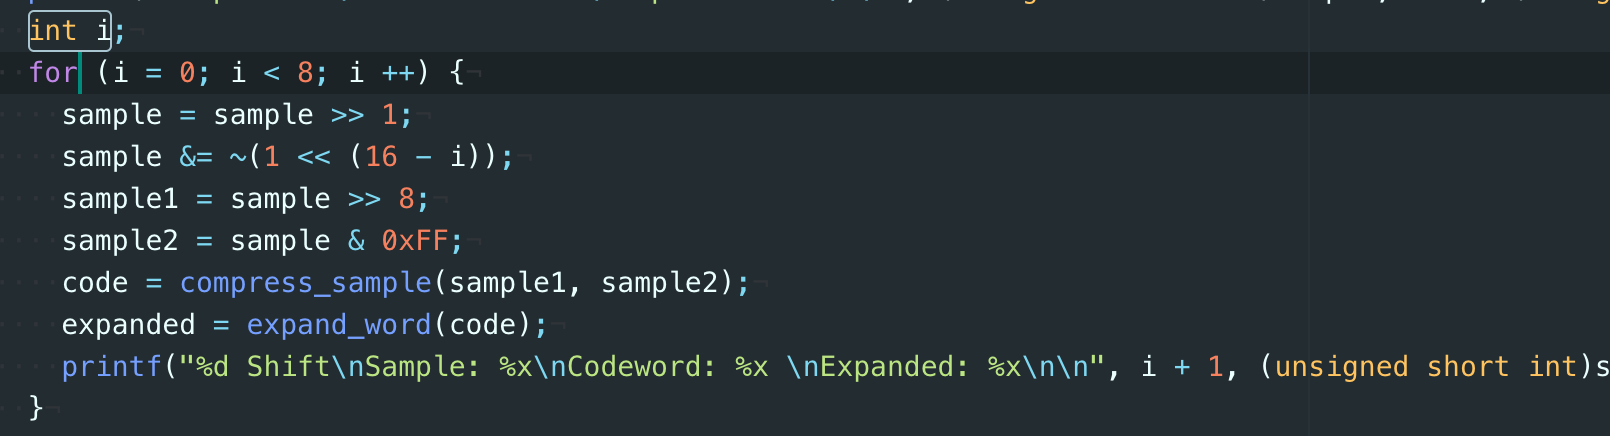
\includegraphics[width=\textwidth]
        {testingLoop.png}
        \caption{\label{fig:my-label} Testing for loop to produce samples to compress}
\end{figure}


\subsection{Original Design}

In the actual implementation of the algorithm, the program would take in a file and write the data into a struct with a place for a header, data and the size of the data. The first thing that was done was removing the head from the original file and placing it in the compressed file. After this was done the data, in the form of 8 bit character data type were compressed, this was done by first getting the sign of the character, the magnitude of the character, the chord and step. After the values were found, they were connected together into one code word and written into the \texttt{Compressed} struct. The header and the compressed data was then written into a file.\\

The sign, step and chord were found through functions calls in the first iteration for the sake of convenience and readability. This was done knowing that it would later have to be optimized, but I thought it would be better to get the algorithm complete and readable before I started optimizing the code. There were multiple different things I did to get more out of readability and harm on speed performance. An example of this can be seen in figure 2, where I used a for loop to cycle through cases to find the leading bit.\\

\begin{figure}[!h]
        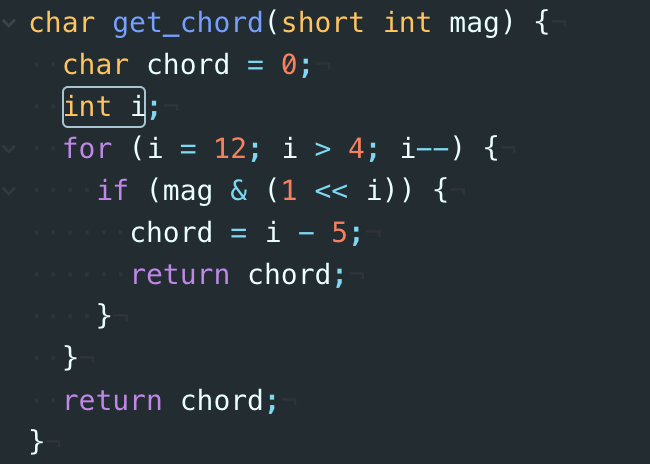
\includegraphics[width=\textwidth ]
        {get_chord_for_loop.png}
        \caption{\label{fig:my-label} For loop used to find the leading one bit.}
\end{figure}
\subsection{Optimizations}

To optimized the code, the parts of the code looked at were the parts that were called the most. All of the parts of code having to do with the compression and expansion could be improved by quite a bit.
\newpage
\end{document}